%--------------------------------------------------------------------
%
% file: cs446_pres.tex
%
% @Author  Iacovos G. Kolokasis
%          Emmanouil Pavlidakis
% @Version 13-05-2018
% @email   kolokasis@ics.forth.gr
%          manospavl@ics.forth.gr
% 
% @brief   Presentatin for the project needed of CS-445 Managed
% Runtime Systems project 

% The theme itself is licensed under a Creative Commons
% Attribution-ShareAlike 4.0 International License. This means that if
% you change the theme and re-distribute it, you must retain the
% copyright notice header and license it under the same CC-BY-SA
% license. This does not affect the presentation that you create with
% the theme.
%
% Downloaded from : https://github.com/matze/mtheme
%
%--------------------------------------------------------------------

%\documentclass[handout,....]{beamer}   % Disable beamer pause
\documentclass[10pt]{beamer}

\usetheme{metropolis}

%--------------------------------------------------------------------
% PACKAGES
%--------------------------------------------------------------------
\usepackage{appendixnumberbeamer}
\usepackage{tabularx}
\usepackage{booktabs}
\usepackage[scale=2]{ccicons}
\usepackage{pgfplots}
\usepgfplotslibrary{dateplot}
\usepackage{xspace}
\usepackage{listings}
\usepackage{textpos}
\newcommand{\themename}{\textbf{\textsc{metropolis}}\xspace}

\setbeamertemplate{footline}{
    \leavevmode%
    \begin{beamercolorbox}[left,wd=.4\paperwidth,ht=2.5ex,dp=1.125ex,leftskip=.3cm, rightskip=.3cm plus1fil]{footline}%
        \href{https://www.csd.uoc.gr/~hy446}{CS446 - Managed RunTime Systems}%
    \end{beamercolorbox}
    %
    \begin{beamercolorbox}[center,wd=.2\paperwidth,ht=2.5ex,dp=1.125ex,leftskip=.3cm,rightskip=.3cm plus1fil]{footline}%
        \centering
        \insertframenumber~\textlatin{of}~\inserttotalframenumber%
    \end{beamercolorbox}%
    %
    \begin{beamercolorbox}[right,wd=.4\paperwidth,ht=2.5ex,dp=1.125ex,leftskip=.3cm,rightskip=.3cm plus1fil]{footline}%
        \hskip2ex plus1fill%
        \href{mailto:manospavl@ics.forth.gr}{\textlatin{$[$ manospavl, }}%
        \href{mailto:kolokasis@csd.uoc.gr}{\textlatin{kolokasis $]$@ics.forth.gr}}
    \end{beamercolorbox}%
}%

%--------------------------------------------------------------------
% TITLE
%--------------------------------------------------------------------
\title{\textlatin{Evaluating the performance of Interpreters\\over various Branch predictors}}
\subtitle{CS-446 -- Managed Runtime Systems}
\date{\today}
\author{Emmanouil Pavlidakis \& Iacovos G. Kolokasis}
\institute{Computer Science Department \\ University Of Crete}
\titlegraphic{\hfill
\includegraphics[height=1.5cm]{figures/UoC_logo.png}}

%--------------------------------------------------------------------
% PRESENTATION SLIDES
%--------------------------------------------------------------------
\begin{document}

{
\maketitle
}

%--------------------------------------------------------------------
% TABLE OF CONTENTS
%--------------------------------------------------------------------
{
\begin{frame}{Contents}
  \setbeamertemplate{section in toc}[sections numbered]
  \tableofcontents[hideallsubsections]
\end{frame}
}

%--------------------------------------------------------------------
% INTRODUCTION
%--------------------------------------------------------------------
\section{Background \& Problem statement}

\begin{frame}{What are Interpreters?}
    \begin{itemize}
    	\item {Directly transforms \& executes program instructions written in a high-level programming language} 
    	\item {Two types of interpreters : }
    	\begin{enumerate}
    		\item {Transform the source code to machine code}
    		\item {Transform the source code to byte code}
    	\end{enumerate}	
        \item {Byte code can be generated: }
	         \begin{itemize}
	         	\item{Statically: Before actual execution (i.e. Java)}
	         	\item{Dynamically: Just before execution (i.e. Python)}
	         	\item{Dynamically: At runtime (i.e. Javascript))}
	         \end{itemize}
    \end{itemize}
    \begin{figure}
	    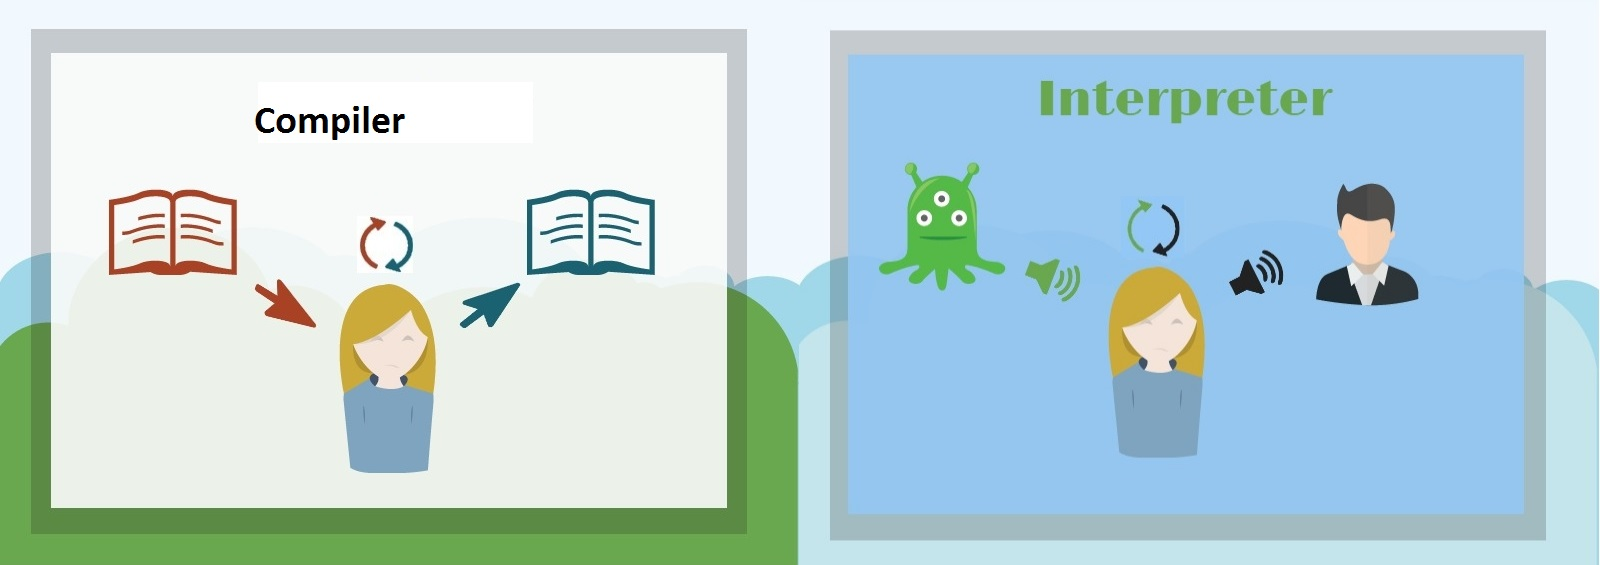
\includegraphics[height=1.5cm]{figures/interVSComp.jpg}
    \end{figure}
\end{frame}

\begin{frame}{Performance issues}
	\begin{itemize}
		\item {Interpreters contain an infinite loop}
			\begin{itemize}
			\item {Fetches, Decodes, and Executes commands}
			\end{itemize}
		\item {Their main overhead derives from this dispatch loop}
		\item {Additional costs come from the switch st.}
				\begin{itemize}
					\item {They causes indirect jump instructions}
					\item {These indirect branches are very difficult to predict}
					\item {Every miss prediction costs almost 20 cycles}
				\end{itemize}
				    \begin{figure}
				    	\begin{textblock*}{3cm}(8.5cm,-2cm)
				    		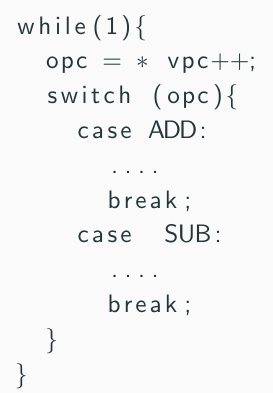
\includegraphics[height=4cm]{figures/dispatchloop.png}
				    	\end{textblock*}
				    	
				    \end{figure}	
	\end{itemize}

\end{frame}

\begin{frame}{Performance }
    \begin{itemize}
        \item{Overheads due to indirect branches}

        \item{We study the properties of current interpreters and
            state-of-the-art branch prediction on bare metal
            architectures}
    \end{itemize}
\end{frame}
%
%\begin{frame}[fragile]
%\begin{lstlisting}
%while(1){
%  opc = * vpc++;
%  switch (opc){
%    case ADD:
%      ....
%      break;
%    case  SUB:
%      ....				
%      break;
%  }	
%}
%\end{lstlisting}
%\end{frame}

%--------------------------------------------------------------------
% Experimental Methodolodgy
%--------------------------------------------------------------------
\section{Experimental Methodolodgy}

%--------------------------------------------------------------------
% Evaluation
%--------------------------------------------------------------------
\section{Evaluation}

%--------------------------------------------------------------------
% Conclusions
%--------------------------------------------------------------------
\section{Conclusions}

%--------------------------------------------------------------------
% Last Slide
%--------------------------------------------------------------------
\begin{frame}[standout] 
    \huge \textlatin{Thanks!}
\end{frame}
\end{document}
